%
\chapter{RTC : Réseau Téléphonique Commuté}
%
%
    \section{Analyse sur un lien}
        \label{seullien} % label pour reference
%
        \subsection{Énoncé}
%
            \paragraph{}
Considérons un lien d'un réseau à commutation de circuits permettant de véhiculer de la voix téléphonique.
%
            \begin{figure}[h]
                \centering
                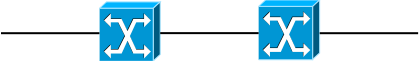
\includegraphics[scale=0.7]{RSC/1-1.png}
                \caption{ Schéma du réseau à commutation de circuit étudié }
                \label{ Schema du reseau a commutation de circuit }
            \end{figure}
%
            \paragraph{}
Chacune des connexions nécessite un débit de $64 \ \text{Kb}.\text{s}^{-1}$ de façon bi-directionnel.
On peut multiplexer simultanément $C$ appels téléphoniques sur ce lien.
%
            \paragraph{}
Le nombre d'utilisateurs est suffisamment grand pour supposer que les arrivées des nouveaux appels suivent une loi de paramètre $\lambda$, les durées des appels sont supposées suivre une loi exponentielle de paramètre $\mu$ avec ($\frac{1}{\mu} = 3 \ \text{minutes}$).
%
%
\clearpage
%
%
        \subsection{Probabilité de blocage d'appel en fonction de la charge $\rho$ et de la capacité $C$}
%
            \[ P(\text{blocage}) = \frac{ \frac{ \rho^C }{ C! } }{ \sum\limits_{i=0}^C \frac{ \rho^i }{ i! } } \]
%
            \begin{center}
                avec $\rho$ la charge en Erlang et $C$ la capacité.
            \end{center}
%
            \paragraph{}
Voici les résultats de ce calcul, obtenus grâce aux calculs réalisés par notre script Python inclus en annexe \ref{seullien-script}
% TODO >>> ici graphique calcul theorique avec k et rho qui changent
            \begin{figure}[h]
                \centering
                \begin{gnuplot}[terminal=epslatex, terminaloptions=color dashed]
                    set xlabel 'Charge (Erlangs)'
                    set ylabel 'Taux de rejet'
                    plot "qnap/partie1/calcul.p1.q1.data" u 2:1 w l t "taux de rejet"
                \end{gnuplot}
                \caption{Résultats de l'étude théorique.}
                \label{pic:p1q1}
            \end{figure}
%
%
\clearpage
%
%
        \subsection{Simulation de cette probabilité de blocage}
%
            \paragraph{}
Pour une charge $10 < \rho < 70$ et pour une capacité $\rho < C < 2*\rho$.
% TODO >>> SIMULATION ici graphique avec k et rho qui changent
        \begin{figure}[h]
            \centering
            \begin{gnuplot}[terminal=epslatex, terminaloptions=color dashed]

            set xlabel 'Charge (Erlangs)'
            set ylabel 'Taux de rejet'
            plot "qnap/partie1/p1.q2.data" u 2:1 w l t "taux de rejet"
            \end{gnuplot}
            \caption{Résultats de l'étude théorique.}
            \label{pic:p1q2}
        \end{figure}
%
%
%
        \subsection{Comparaison des taux de blocage expérimentaux et théoriques}
            \paragraph{}
Blablabla 3
%
%
    \clearpage
%
%
%
    \section{Analyse sur un réseau de trois commutateurs}
%
        \subsection{Énoncé}
%
            \paragraph{}
Désormais, nous considérons le réseau composé de 3 noeuds.
%
            \begin{figure}[h]
                \centering
                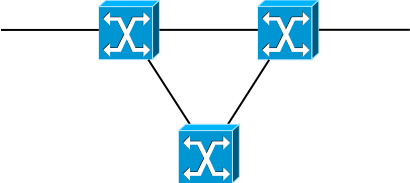
\includegraphics[scale=0.6]{RSC/1-2.png}
                \caption{ Schéma du réseau à 3 commutateurs de circuit étudié }
                \label{ Schema du reseau a 3 commutateurs de circuit }
            \end{figure}
%
            \paragraph{}
Les arrivées sont supposées Poissonniennes sur chacun des nœuds et le trafic se répartit équiprobablement entre les différents nœuds.
Les durées des appels sont supposées exponentielles de même paramètre que dans la première partie (1-a).
Nous ne considérons pas les appels locaux ni les appels qui n'aboutissent pas (absence).
%
%
    \clearpage
%
%
        \subsection{Probabilités de blocage avec le chemin de débordement en cas de saturation du chemin direct}
%
            \paragraph{}
Blablabla 4.
Avec un canal de débordement on obtient donc une capacité doublée, il n'y plus de blocage ... ?
%
        \subsection{Comparaison des résultats avec la partie \ref{seullien}}
        % (on choisira donc des charges de trafic et des capacités de liens équivalentes)
Blablabla 5
    % TODO >>>
    % ici graphique simulation et calculs ??
    % TODO <<<
%~ \begin{figure}
    %~ \centering
    %~ \begin{gnuplot}[terminal=epslatex, terminaloptions=color dashed]

    %~ set xlabel 'Charge (\%)'
    %~ set ylabel 'Taux de rejet'
    %~ plot "qnap/partie2/p2.q3.data" u 1:2 t "minT",\
        %~ "qnap/partie2/p2.q3.data" u 1:3 t "maxT",\
        %~ "qnap/partie2/p2.q3.data" u 1:4 w l t "moyenne temps traitement",\
        %~ "qnap/partie2/p2.q3.data" u 1:5 t "minA" axes x1y2,\
        %~ "qnap/partie2/p2.q3.data" u 1:6 t "maxA" axes x1y2,\
        %~ "qnap/partie2/p2.q3.data" u 1:7 w l t "moyenne nb paquets en attente" axes x1y2
    %~ \end{gnuplot}
    %~ \caption{This is a simple example using the epslatex-terminal.}%
    %~ \label{pic:epslatex}%
%~ \end{figure}
%
%
    \clearpage
%
%
        \subsection{Problèmes à très forte charge !}
%
            \paragraph{}
Une solution consiste à n'utiliser le chemin de débordement que lorsque celui-ci n'est pas très encombré, c'est à dire en dessous d'un certain seuil d'occupation sur chacun des liens.
Cela revient donc à laisser une marge M aux appels directs.
%
%
            \subsubsection{Commentaires}
%
                \paragraph{}
Blablabla 6
%
%
            \subsubsection{Simulation en prenant une marge comprise entre 1 et 3}
%
                \paragraph{}
Blablabla 7
% TODO >>> ici graphique simulation
            %~ \begin{figure}
                %~ \centering
                %~ \begin{gnuplot}[terminal=epslatex, terminaloptions=color dashed]

                %~ set xlabel 'Charge (\%)'
                %~ set ylabel 'Taux de rejet'
                %~ plot "qnap/partie2/p2.q3.data" u 1:2 t "minT",\
                    %~ "qnap/partie2/p2.q3.data" u 1:3 t "maxT",\
                    %~ "qnap/partie2/p2.q3.data" u 1:4 w l t "moyenne temps traitement",\
                    %~ "qnap/partie2/p2.q3.data" u 1:5 t "minA" axes x1y2,\
                    %~ "qnap/partie2/p2.q3.data" u 1:6 t "maxA" axes x1y2,\
                    %~ "qnap/partie2/p2.q3.data" u 1:7 w l t "moyenne nb paquets en attente" axes x1y2
                %~ \end{gnuplot}
                %~ \caption{This is a simple example using the epslatex-terminal.}%
                %~ \label{pic:epslatex}%
            %~ \end{figure}
%
%
    \clearpage
%
